\documentclass[12pt]{beamer}
\usepackage[T1]{fontenc}
\usepackage{beamerthemeHannover, graphicx, amsmath, amssymb, multicol}
\usepackage{textcomp} \usepackage{verbatim}
\usepackage{listings}
\setbeamercolor{sidebar}{use=structure,bg=red!50!yellow}
\lstset{language=perl}

\title{Introduction to Dist::Zilla for Newbies}
\author[@dukeleto]{Jonathan "Duke" Leto}
\date{}

\begin{document}

\frame{
    \titlepage
    \begin{center}
    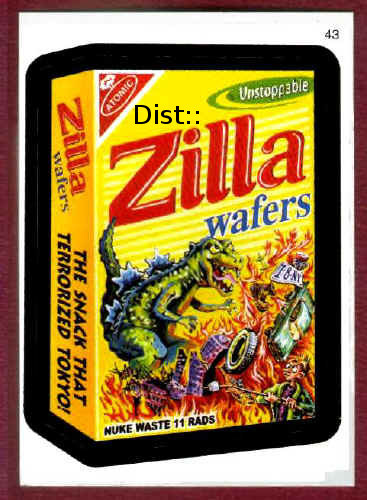
\includegraphics[width=105px, height=135px]{zilla.jpg}
    %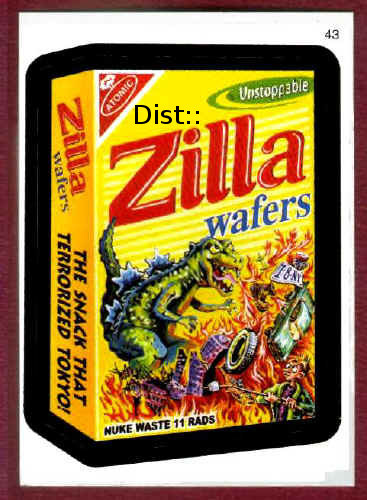
\includegraphics{zilla.jpg}
    \end{center}
}

\frame{
    \frametitle{What is Dist::Zilla?}

    Dist::Zilla automates boring stuff so you can concentrate on fun stuff.
}

\frame{
    \frametitle{Why is Dist::Zilla Useful?}
    \begin{itemize}
        \item Automate listing prereqs(!)
        \item Automate creating tarballs
        \item Automate uploading to CPAN
        \item Automate "version bumping", both in the source and in version control
        \item Automate creating new project skeletons
        \item Automate creating Debian packages
        \item Has many plugins to do other stuff
    \end{itemize}
}

\frame{
    \frametitle{Install Dist::Zilla}
    \begin{itemize}
        \item cpanm Dist::Zilla
        \item dzil setup \# creates \$HOME/.dzil
    \end{itemize}
}

\frame{
    \frametitle{Create a new project skeleton with dzil}
    \begin{itemize}
        \item dzil new My::Awesome::Thingy
    \end{itemize}
}

\frame{
    \frametitle{Other common dzil tasks}
    \begin{itemize}
        \item dzil build
        \item dzil test
        \item dzil release \# send to CPAN
    \end{itemize}
}

\frame{
    \frametitle{dzil and dependencies}

    \begin{itemize}
        \item dzil authordeps | cpanm
        \item dzil listdeps   | cpanm
    \end{itemize}
}

\frame{
    \frametitle{Real Life dist.ini}
    App::Beeminder::Hook
    \tiny{
        \lstinputlisting{app_beeminder_hook_dist.ini}
    }
}

\frame{
    \frametitle{Cool Plugins}
    \begin{itemize}
        \item Dist::Zilla::Plugin::HelpWanted
        \item Dist::Zilla::Plugin::Covenant
        \item Dist::Zilla::Plugin::Moz
        \item Dist::Zilla::Plugin::Mercurial
        \item Dist::Zilla::Plugin::Twitter
    \end{itemize}
}

\frame{
    \frametitle{ More Info }
    \begin{itemize}
        \item \#distzilla on irc.perl.org
        \item dzil.org
    \end{itemize}
}

\frame{
    \frametitle{ Thanks! }
    \begin{itemize}
        \item Portland Perl Mongers
        \item RJBS, for writing Dist::Zilla
    \end{itemize}
}

\frame{
    \frametitle{ Stalk Me }
    \begin{center}
        \begin{itemize}
           \item http://dukeleto.pl
           \item @dukeleto
           \item dukeleto on the IRCwebs
        \end{itemize}
    \end{center}
}
\end{document}
